% Generated by thesis/ch7/exp2/networks.py -- do not edit by hand.
\begin{sidewaysfigure}
  \centering
  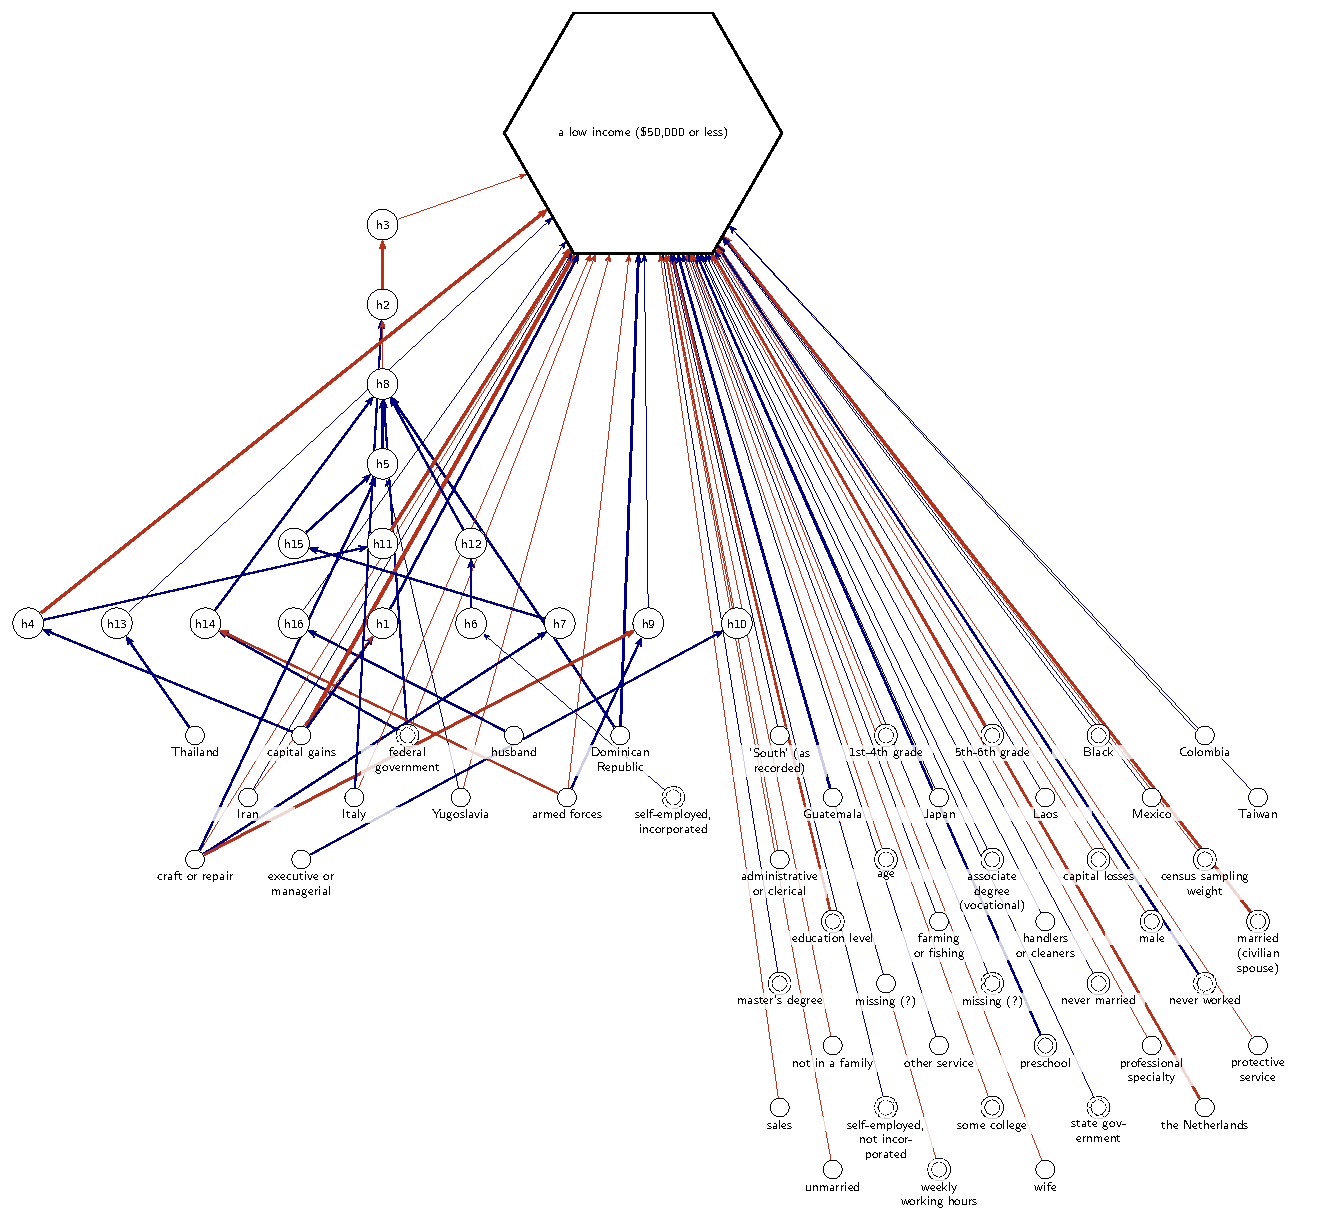
\includegraphics[width=\textheight,height=0.78\textwidth,keepaspectratio]{figures/exp2/networks/adult-s1-raw}
  \caption{Adult, seed 1 (adult-s1): the network as trained, before any explanation, in full. Inputs at the bottom (every input column its own node), hidden units by depth, the output at the top; 50 of 107 input columns are connected, with 16 hidden units and 80 enabled connections. Blue: positive weight (raises the score); red: negative weight (lowers it); thicker: larger weight. Orange outline and up arrow: raises the final prediction; teal and down arrow: lowers it; grey and double arrow: depends. Not used (no connection; 57 columns): local government, private, without pay, 10th grade, 11th grade, doctorate, high-school graduate, professional school degree, 12th grade (no diploma), 7th-8th grade, 9th grade, associate degree (academic), bachelor's degree, divorced, married to a member of the armed forces, married, spouse absent, separated, widowed, missing (?), technical support, transport or moving, machine operator or inspector, private household service, other relative, own child, American Indian or Eskimo, Asian or Pacific Islander, other race, White, Cambodia, France, Germany, Greece, Haiti, Honduras, Hong Kong, Hungary, India, Canada, Ireland, Jamaica, Nicaragua, outlying US territories (Guam, US Virgin Islands), Peru, China, the Philippines, Poland, Portugal, Puerto Rico, Scotland, Trinidad and Tobago, the United States, Vietnam, Cuba, Ecuador, El Salvador and England.}
  \label{fig:exp2-net-adult-s1-raw}
\end{sidewaysfigure}
